%\chapter*{Conclusions}

\chapter[Analysis and Conclusions]{Analysis and Conclusions}
\label{chap:Conclusions}

\noindent This chapter presents the results and conclusions of the search 
for \Zprime~bosons in the di-hadronic tau channel, using proton-proton 
collisions at a \centermassenergy~of 13 \TeV, with the data 
collected by the CMS experiment during 2016, which have 35.9 fb$^{-1}$ of 
integrated luminosity. This analysis is currently \textit{unblinded}, i.e., the
CMS Collaboration has approved to explore with the real data the region where 
the \Zprimetotautau~is expected. In order to avoid any bias 
in the analysis and to ensure objectivity, the CMS Collaboration 
does not allow to explore the signal region with real data until
all the procedures have been validated; this means that the whole 
procedure described in Chapter \ref{chap:Analysis}, as well as the procedures 
performed for the other di-tau channels (\tauh\taumu, \tauh\taue~and \taumu\taue), have already 
been approved by the Collaboration. However, the results using real data 
are still being reviewed internally and, therefore, they are 
not included in this document. Instead, expected exclusion 
limits have been calculated (see Section \ref{sec:Analysis}), showing that
the sensitivity in the di-hadronic tau channel has improved over the one 
obtained with the combination of all four channels, using the data 
collected by CMS during 2015. 

\section{Analysis}
\label{sec:Analysis}

\noindent The exclusion limit calculation is based on the assumption that any 
\Zprime~existence is discarded. This is achieved by generating 
\textit{pseudo-data} samples, which are constructed with the 
background-only hypothesis, and performing the calculation as 
if they were real data. The quantity of interest in order to set 
the exclusion limit is $\sigma \cdot B$, where $\sigma$ is 
the cross-section for the \Zprime~production ($pp \rightarrow$ \Zprime) 
and $B$ is the branching ratio of this boson decaying into taus (\Zprimetotautau);
indeed, this quantity is proportional the expected number of signal events, and it can 
be compared with the ``observed'' events (using the pseudo-data). The compatibility
of the ``observed'' data and the signal expectation on the effective visible mass
distribution, which provides the best discrimination between signal and background,
is quantified using a modified frequentist approach, known as CL$_{s}$ method \cite{CLs1Cowan,CLs2}. This 
statistical method, as well as the expected exclusion 
limits calculation, are presented in this section. 

\subsection{Statistical Method}
\label{subsec:statisticalmethod}

\noindent With the purpose to characterize the non-observation of 
the signal and to set the exclusion limit, one defines the null 
hypothesis H$_{0}$, which describes the signal-plus-background 
processes. This is tested against an alternative hypothesis
H$_{1}$, which is based on the background-only assumption. In order to 
quantify the compatibility of the ``observed'' data with a 
given hypothesis, there are two approaches: the Bayesian 
and the frequentist approaches. They differ in the way in which the 
probability is defined. For the Bayesian approach, the probability can 
be interpreted as the ``degree of belief'' of the result for a given 
experiment. For the frequentist approach, which is used in
this analysis, it can be interpreted as the 
probability to obtain a given measurement after 
repeating experiment many times. \\

\noindent In the particle physics community the frequentist approach, based on a 
binned likelihood ratio, is widely used to establish, or to exclude,
the existence of a new phenomenon. In this analysis, the 
calculation of the exclusion limit is obtained by using each bin for
the \mass~distribution in order to evaluate the likelihood per bin. Their 
combination results in the upper limit on the cross-section, for a given 
\Zprime~mass point, where the level of compatibility of the 
``observed'' data with a given hypothesis is quantified by the 
confidence level (CL). Since it is a convention, 95$\%$ CL for excluding 
the signal is used in this analysis. \\

\noindent In the following, the signal and background yields 
will be denoted as $s$ and $b$, respectively. Their predictions are 
subject to systematic uncertainties (see Section \ref{sec:Systematics}) that 
can be included in the exclusion limit calculation as 
nuisance parameters ($\theta$). Then, the signal and background
are functions of the nuisance parameters ($s(\theta)$ and $b(\theta)$). \\

\noindent The likelihood function is given by:
% , or probability to measure the \mass~yields per bin in a single experiment,

\begin{equation} \label{eq:likelihood}
 \mathcal{L}(\theta) = \prod_{i=1}^{N-bins}L_{i}(s_{i},b_{i},n_{i};\theta) \; ,
\end{equation}

\noindent where $\theta$ is the set of nuisance parameters 
and $L_{i}(s_{i},b_{i},n_{i};\theta)$ is the likelihood function for the i-th bin, 
which represents the probability function for obtaining an ``observed'' data yield in 
the i-th bin given an hypothesis H. Since the 
number of independent results is large and the cross-section for a 
signal event is very low, compared with the cross-section for background 
events, the probability density is a Poisson distribution:

\begin{equation} \label{eq:Poisson}
 L_{i}(s_{i},b_{i},n_{i};\theta) = \frac{(s_{i}+b_{i})^{n_{i}}}{n_{i}!}e^{s_{i}+b_{i}} \; ,
\end{equation}

\noindent then, $L_{i}(s_{i},b_{i},n_{i};\theta)$ is the Poisson probability of observing
$n_{i}$ events in data in the i-th bin, given the hypothesis H. As a result, $\mathcal{L}_{s+b}(\theta)$ is 
the product of $N$ Poisson probabilities of observing ${n_{i}}$ `` events in the data, for all 
the bins, where ${s_{i}+b_{i}}$ events are expected, where $N$ is the number of bins. And $\mathcal{L}_{b}(\theta)$ is the product 
of $N$ Poisson probabilities of observing ${n_{i}}$ events in data, where only background 
events are expected.\\

\noindent These likelihood functions are the result of a 
single measurement of signal and background yields 
in the \mass~distribution; therefore, $s_{i}$ and $b_{i}$ are the mean values, 
in the i-th bin, of the distribution of all possible $s_{i}$ and $b_{i}$ values that 
could have been obtained if the experiment would have been repeated several times. Instead 
of repeating the experiment several times is not possible, an 
ensemble of experiments is simulated. This ensemble is obtained generating 
pseudo-data samples with the background-only hypothesis; each experiment of this ensemble
provides an independent new possible result. As a consequence, a probability 
distribution is obtained for the $s_{i}$ and $b_{i}$ yields, allowing to consider 
any fluctuation in data and, resulting in an improvement on 
the sensitivity of the statistical method. \\

\noindent The CL${s}$ method tests the null hypothesis 
(signal plus backgrounds) against the background-only hypothesis through 
the likelihood ratio (LR). The LR is the best discriminator between both hypotheses,
and it is given by \cite{CLs1Cowan}:

\begin{equation}\label{eq:LR}
LR = -2 \ln \frac{\mathcal{L}_{s+b}(\theta^{''})}{\mathcal{L}_{b}(\theta^{'})} \; .
\end{equation}

\noindent From the equation it is possible to infer that ``observed'' events with $LR > 0$ are more 
compatible with the background-only hypothesis H$_{1}$ than with the signal-plus-background 
hypothesis H$_{0}$. Here $\theta^{''}$ and $\theta^{'}$ denote the value of the 
systematic uncertainties that maximizes the likelihood for H$_{0}$ and H$_{1}$
respectively. This procedure is known as binned maximum likelihood for the 
signal-plus-background and background only hypotheses. The dependence on the nuisance parameters 
is reflected as a broaden likelihood distribution, compared with the one if they were fixed. This 
represents a loss of sensitivity in the analysis due to the systematic uncertainties \cite{CLs1Cowan}.\\

\noindent As mentioned in section \ref{sec:Systematics}, the systematic uncertainties can 
affect the normalization or the shape of the \mass~distribution. They are included 
in the likelihood calculation through an MC numerical integration method over all the 
nuisance parameters. In the case when a systematic uncertainty affects the normalization,
such as the one of the tau trigger, the nuisance parameters are generated with a 
logarithmic normal probability density function. In the case when a systematic
uncertainty affects the shape, such as the one of the high-\pt~tau identification, the nuisance
parameters are generated with a Gaussian probability density function 
for the \mass~spectrum uncertainty. \\

\noindent Once the systematic uncertainties are included, the likelihood distribution 
(equation \ref{eq:likelihood}) is used to obtain the 95$\%$ CL upper limit 
for the signal cross-section. The confidence level of the upper limit, 
using the CL$_{s}$ method is given by \cite{CLs1Cowan}:

\begin{equation}\label{eq:CL}
 \textrm{CL}_{s} = \frac{CL_{s+b}}{CL_{b}} \; ,
\end{equation}

\noindent where CL$_{s+b}$ quantifies the compatibility of the ``observed'' data with the
signal-plus-background hypothesis and CL$_{b}$ quantifies the compatibility of the ``observed'' data 
with the background-only hypothesis. In this method the quantity  CL$_{s}$ must be less or equal 
than 0.05 in order to set the 95$\%$ CL in the exclusion limit calculation. \\

\noindent This procedure results in the exclusion limit calculation at a given CL for
an specific \Zprimetotautau~channel. This procedure was performed 
for the di-hadronic tau channel, as well as for the other 
channels: \tauh\taumu, \tauh\taue~and \taumu\taue. Therefore, in order 
to set an exclusion limit for the search for \Zprime~bosons in 
the di-tau final state the results must be combined. Even though 
a high sensitivity is reached in this analysis, a considerable
improvement on the sensitivity is achieved by combining 
the results of the four di-tau channels. This can be done by computing
a total binned likelihood:

\begin{equation}
 \mathcal{L}_{tot} = \mathcal{L}(\tau_{h},\tau_{h}) \times \mathcal{L}(\tau_{h},\tau_{\mu}) \times \mathcal{L}(\tau_{h},\tau_{e}) \times \mathcal{L}(\tau_{\mu},\tau_{e}) \; .
\end{equation}



% They are given by:
% 
%  \begin{equation}
%   \begin{aligned}
%     \textrm{CL}_{s+b} &= P(LR_{s+b} < LR_{observed}) &= N(LR_{s+b} < LR_{observed}) \; , \\
%     \textrm{CL}_{b} &= P(LR_{b} < LR_{observed}) &= N(LR_{s+b} < LR_{observed})  \; .
%   \end{aligned}
%  \end{equation}

\subsection{Exclusion Limit Calculation}
\label{subsec:ExclusionLimits}

\noindent An expected exclusion limit at 95$\%$ CL is set 
on $\sigma (pp\rightarrow\textrm{Z}^{\prime}) \cdot B(\textrm{Z}^{\prime}\rightarrow\tau\tau)$ using the 
method described above. In summary, the calculation of the exclusion limit
is performed using the \mass~distribution in order to construct the 
binned maximum likelihood for the signal-plus-background and background-only 
hypotheses. The binned likelihood is the product of the Poisson probabilities (equation \ref{eq:Poisson}). The systematic 
uncertainties are included in the calculation considering a logarithmic normal 
probability function for normalization parameters, and a Gaussian probability 
function for mass-spectrum shape uncertainties. Finally, the exclusion limit calculation
is performed with the modified frequentist approach, known as the CL$_{s}$ method, which uses 
the likelihood ratio discriminator (equation \ref{eq:LR}) in order to set the limits 
on the signal cross-section at the level of accuracy desired (equation \ref{eq:CL}). Note 
that the results with real data are not public yet, and instead the limits were calculated by
treating pseudo-data, based on background-only hypothesis, as if they were real data. \\

\noindent The statistical procedure described above is performed using 
the CMS Higgs limit calculation tool \textit{Combine} \cite{CombinedTool}. The input
of the tool are the so-called \textit{data cards}, which include the total 
yields and the \mass~distributions for signal and backgrounds, as well
as their systematic uncertainties. \\

\noindent The \Zprime~search is model-independent since it is based of the observation
of an excess in the high spectrum of effective visible mass distribution; this means that 
the signal acceptance estimation presented in Chapter \ref{chap:Analysis}
is independent of the model. If a signal evidence were found, the signal cross-section 
could point towards a particular BSM scenarios. Similarly, the 
exclusion limit calculation on the signal cross-section depends
on the model. Exclusion limits are calculated for the \ZprimeSSM~boson,
considering the cross-section presented in Table \ref{tab:signal_samples}, and 
for the \ZprimeTAT~boson, considering that its cross-section is about one third of 
the one of the SSM model. As a result of the exclusion limit calculation performed for this 
analysis, we expect to exclude \ZprimeSSM~and \ZprimeTAT~bosons (decaying into two hadronic taus)
for masses below 2.7 \TeV~and 2.2 \TeV, in the case in which no signal is observed.\\

\noindent Figure \ref{fig:ExclusionLimitstauh} shows the expected limits (dash line) 
and the leading order theoretical cross-section for \ZprimeSSM~and \ZprimeTAT~(red and blue lines),
in the di-hadronic tau channel. The exclusion limits are presented as a function of 
the effective visible mass. The bands represent the 1$\sigma$
and 2$\sigma$ deviations from the expected limits. The bands were obtained 
using the pseudo-data samples, based on the background-only hypothesis, described 
in the previous section. Note that the exclusion limit on the \Zprime~mass
is determined at the point in which the expected limit on the cross-section 
exceeds the theoretical one. For completeness, the expected exclusion limits 
for the other channels are presented in Figure \ref{fig:ExclusionLimits}. The 
expected exclusion limits for the \ZprimeSSM~boson in the \tauh\taumu, \tauh\taue~and \taue\taumu~channels
are 2.65 \TeV, 2.6 \TeV~and 1.75 \TeV, respectively \cite{AN2018}. 
 
 \begin{figure}[ht]
  \begin{center}
  \captionsetup[subfloat]{farskip=0pt,captionskip=0.0cm,labelformat=empty}
  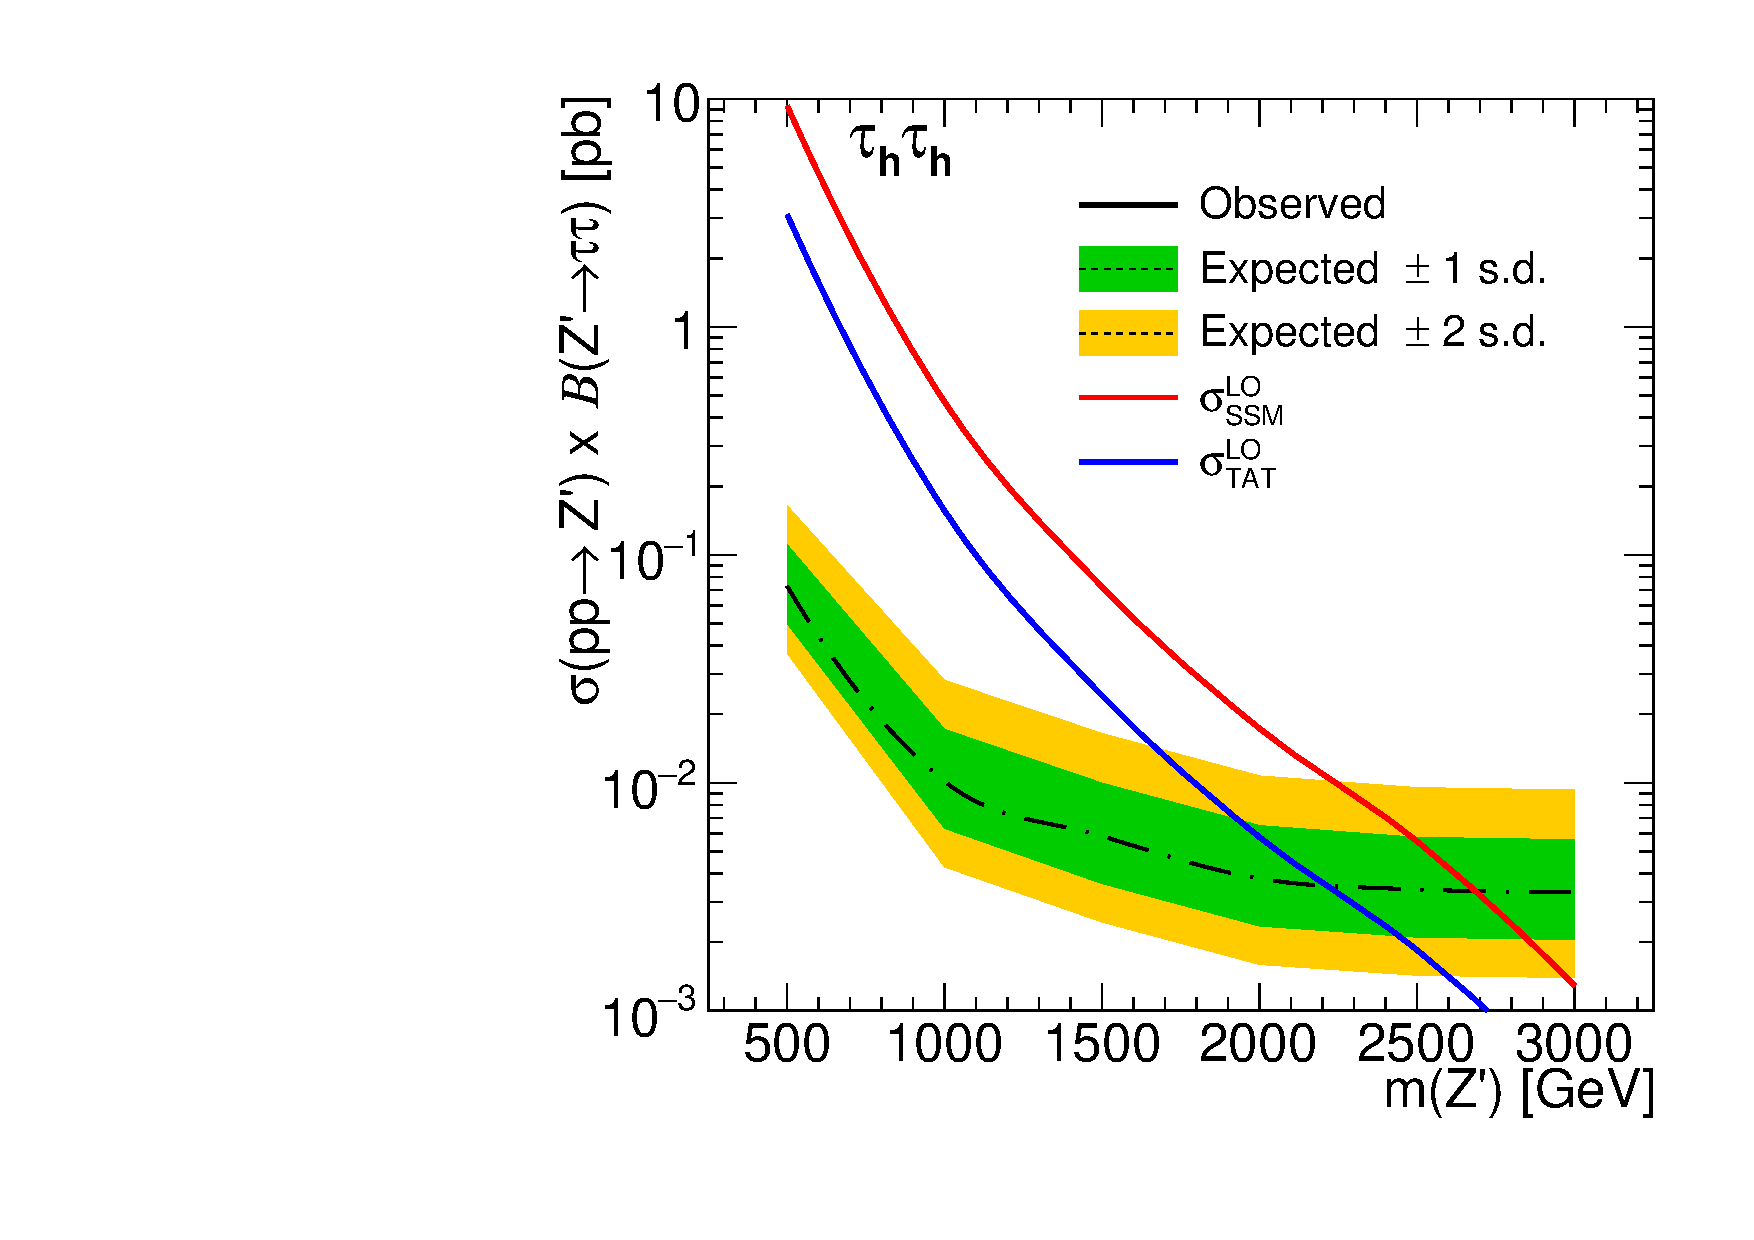
\includegraphics[clip,width=0.5\textwidth]{figuras/Conclusions/tt_Limits.pdf}
  \end{center}
  \caption{Expected exclusion limits at the 95$\%$ CL on $\sigma (pp \rightarrow \textrm{Z}^{\prime}) \cdot B(\textrm{Z}^{\prime} \rightarrow \tau\tau)$,
  for the \tauh\tauh~channel, as a function of the \Zprime~mass. The result is compared 
  with the leading order theoretical expectations for the SSM and TAT models.}
 \label{fig:ExclusionLimitstauh}
 \end{figure}

\begin{figure}[ht]
\begin{center}
\captionsetup[subfloat]{farskip=0pt,captionskip=0.0cm,labelformat=empty}
% \resizebox{\textwidth}{8.8cm}{
%   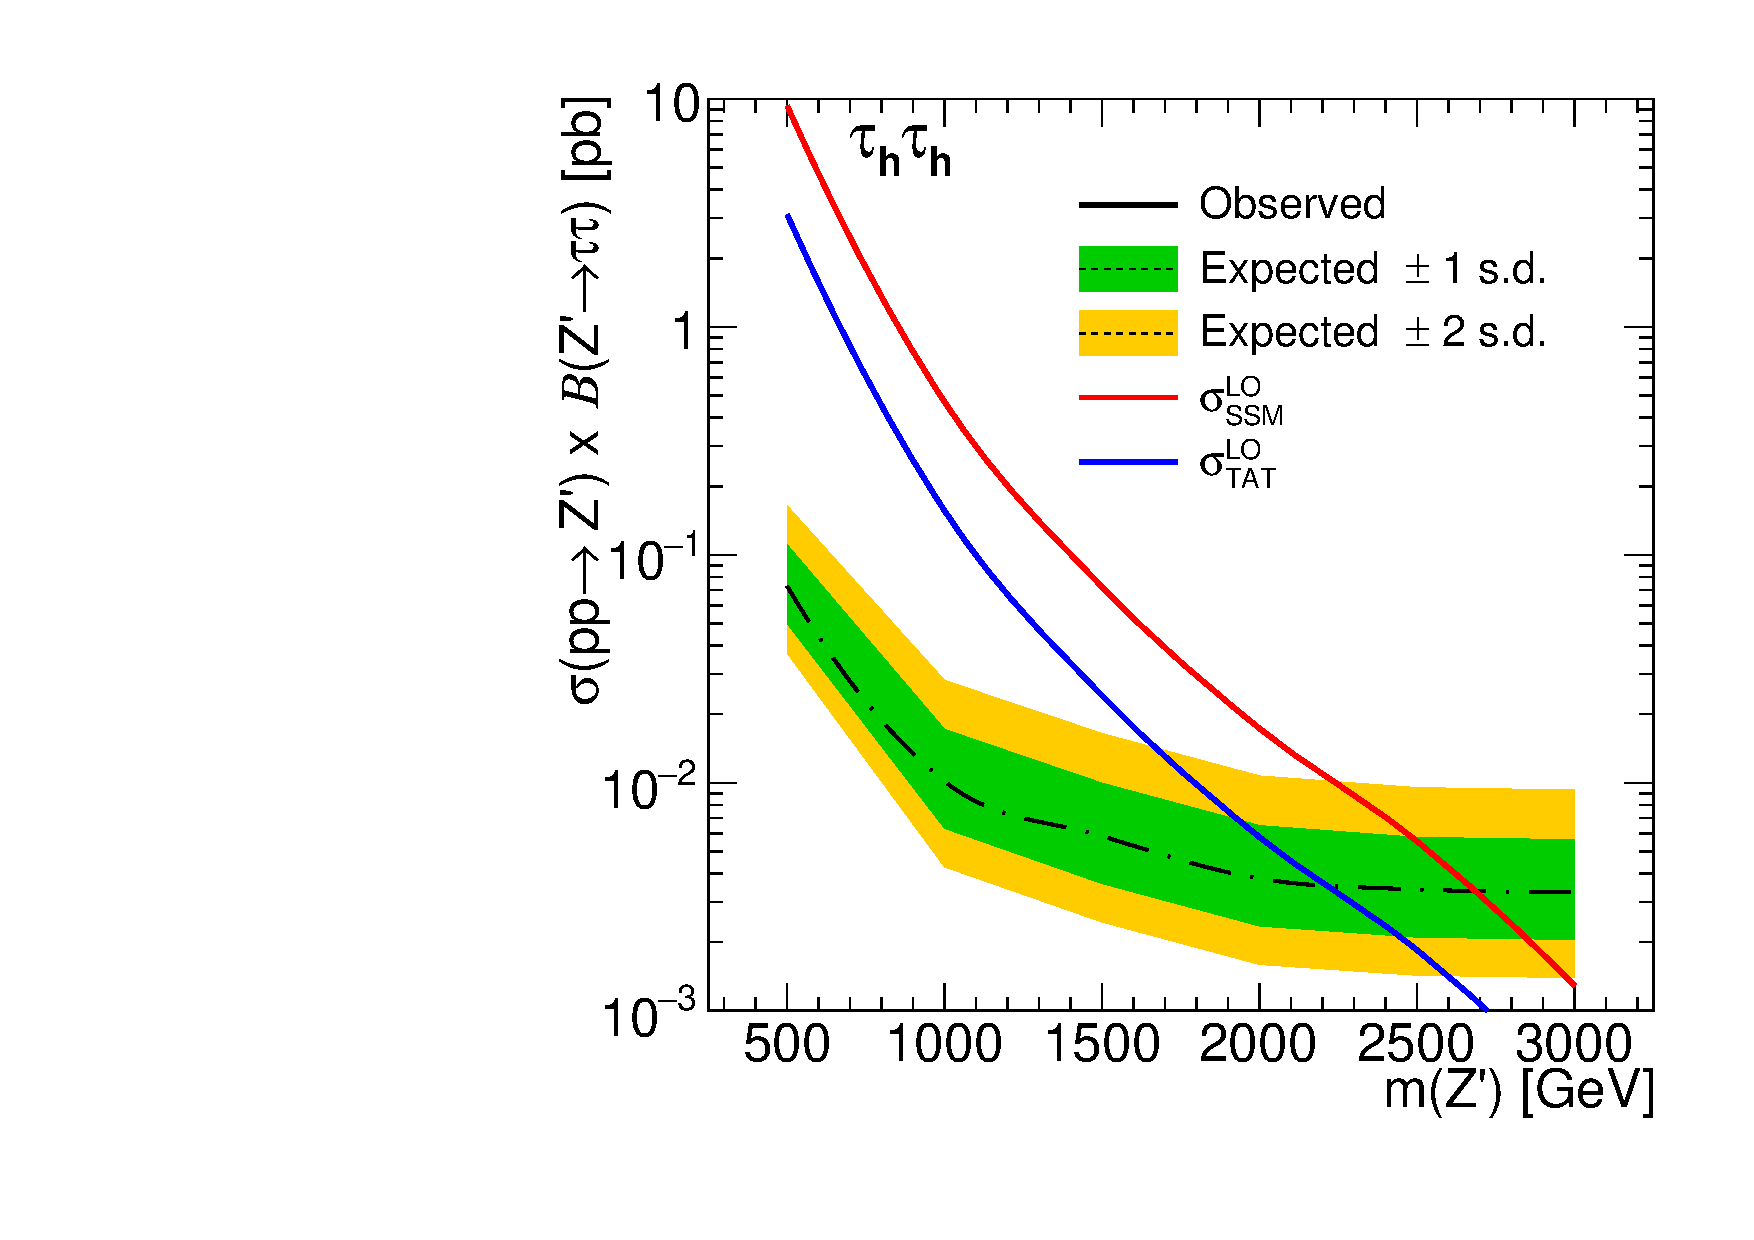
\includegraphics[clip,width=0.45\textwidth]{figuras/Conclusions/tt.pdf}
  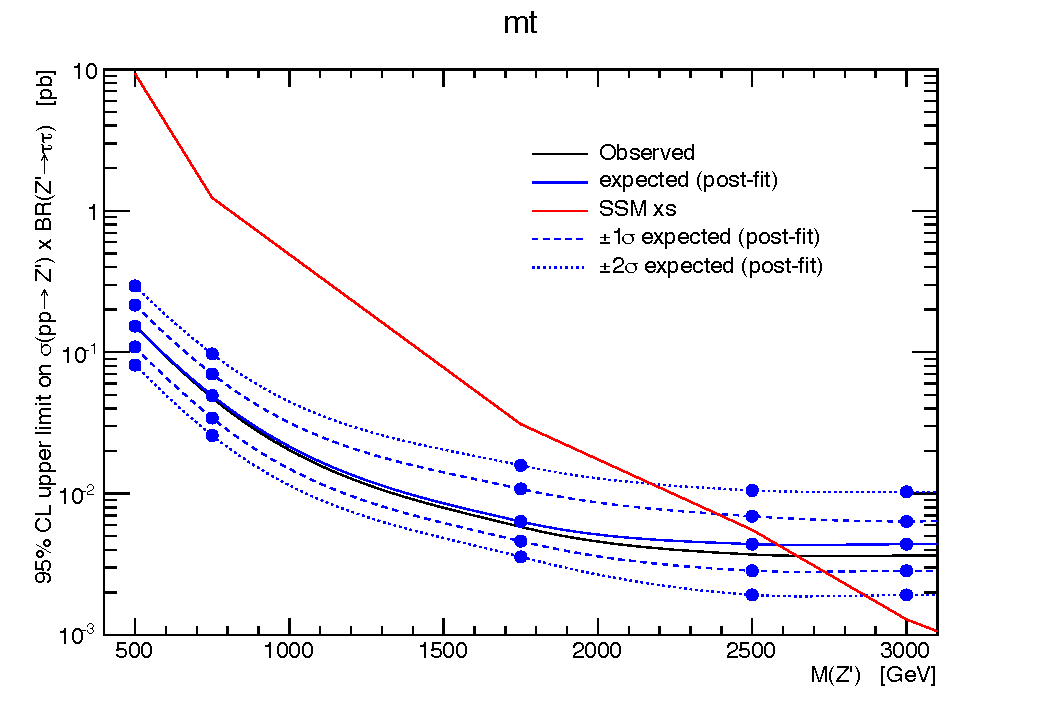
\includegraphics[clip,width=0.45\textwidth]{figuras/Conclusions/mt.pdf}
  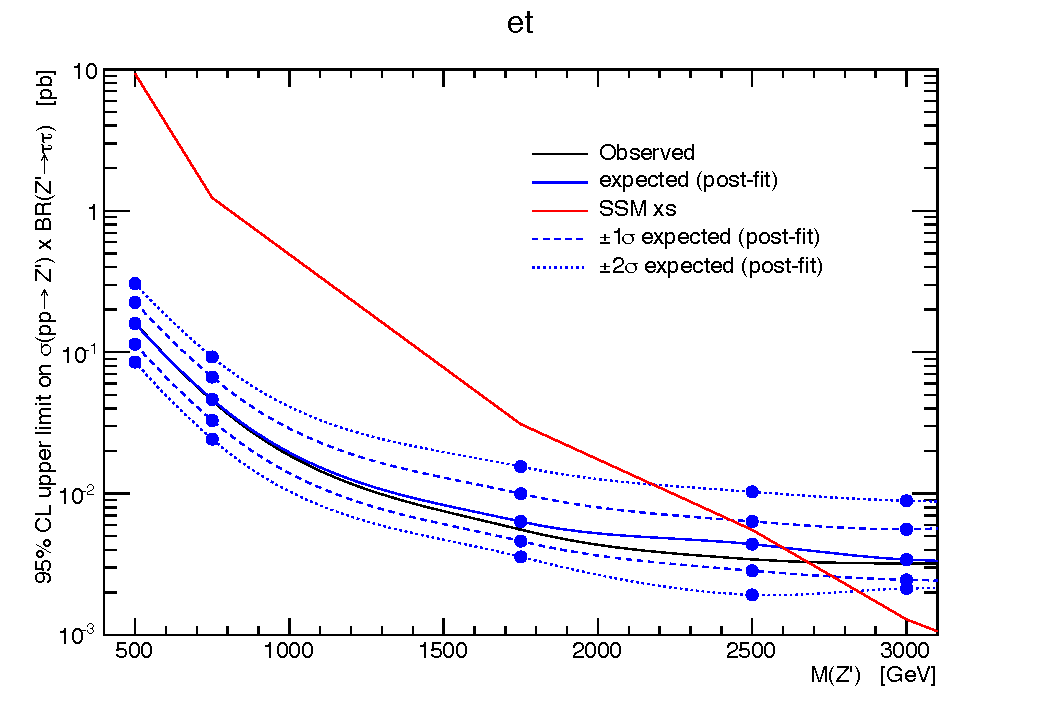
\includegraphics[clip,width=0.45\textwidth]{figuras/Conclusions/et.pdf}\hfill
  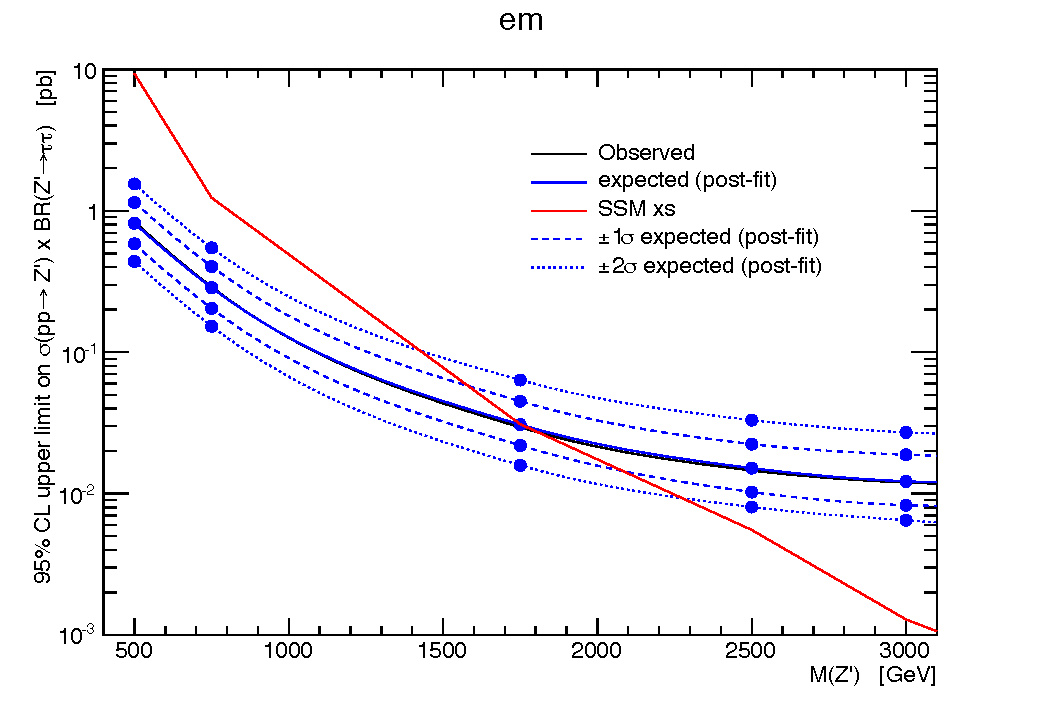
\includegraphics[clip,width=0.45\textwidth]{figuras/Conclusions/em.pdf}	
% }
\end{center}
\caption{Expected exclusion limits at the 95$\%$ CL on $\sigma (pp\rightarrow\textrm{Z}^{\prime}) \cdot B(\textrm{Z}^{\prime}\rightarrow\tau\tau)$ as 
a function of the \Zprime~mass. The result is compared with the leading order theoretical expectations for the SSM and TAT models. The figure 
shows the results for the \tauh\taumu~(top left), \tauh\taue~(top right) and \taue\taumu~(bottom) channels.}
\label{fig:ExclusionLimits}
\end{figure}

\section{Analysis of Results}
\label{AnalysisResults}

\noindent As already mentioned, the search for \Zprime~bosons in the di-hadronic 
tau channel, using the data collected by CMS during 2016, has set 
expected exclusion limits for the \ZprimeSSM~and the \ZprimeTAT~for masses 
below 2.7 \TeV~and 2.2 \TeV, respectively. This section presents 
a comparison of the results with the ones obtained in the other 
di-tau channels (see Section \ref{CMS2016}). Additionally, the results are 
compared with the most recent searches for \Zprime~bosons performed by CMS and 
ATLAS (see Sections \ref{CMS2015} and \ref{ATLAS}). 

\subsection{Comparison with Other Channels}
\label{CMS2016}

Figures \ref{fig:ExclusionLimitstauh} and \ref{fig:ExclusionLimits} show the 
expected exclusion limit, calculated for the di-hadronic tau channel and for 
the other di-tau final states, using the data collected by CMS during 2016. Note that 
the expected exclusion limit for the \ZprimeSSM~mass 
in the \tauh\tauh~channel (2.7 \TeV) is similar to the ones obtained for the 
\tauh\taumu~and \tauh\taue~channels (2.65 \TeV~and 2.6 \TeV). The results are 
similar since, even though the di-hadronic tau channel has the highest 
branching ratio (42$\%$) among the di-tau channels, it also has 
highest QCD contamination that lowers its sensitivity. Since in the di-hadronic case, 
the tau sample is contaminated by QCD-jets, it makes the \tauh\tauh~signal less clean 
than the \tauh\tauell. Another reason that affects the 
sensitivity of the di-hadronic tau channel is the systematic uncertainty 
associated to the identification of high-\pt~taus; this 
source of systematics represents $\sim$25$\%$ uncertainty for a \Zprime~mass of 2 \TeV, while 
it represents $\sim$10$\%$ uncertainty on the same \Zprime~mass
in the case of the \tauh\tauell~channels. Note that, although the \taue\taumu~final 
state is the cleanest channel, due to the low contamination of QCD processes
and the high efficiency of the light lepton reconstruction, the search in this channel sets
the lowest exclusion limit due to its small branching ratio ($6.2\%$). 


% one or both of the taus
% the two taus 
% This is caused because the probability 
% of misidentifying a QCD-jet as a hadronic tau is at least one 
% order of magnitude higher than the probability for a QCD-jet misidentifying 
% an electron or a muon; this makes the \tauh\tauell~signatures cleaner. 

%  for \Zprime~bosons using 2015 data in CMS

\subsection{Comparison with previous CMS Searches}
\label{CMS2015}

In Chapter \ref{chap:Zp} (Table \ref{tableCMSATLASditau}) the results of previous
searches performed by CMS were presented. An exclusion limit of 1.4 \TeV~for 
\ZprimeSSM~was set with the data at 7 \TeV$/$8 \TeV~(Run I). During Run II, at 13 \TeV, initial exclusion 
limits were set for \ZprimeSSM~and \ZprimeTAT~of 2.1 \TeV~ 1.7 \TeV, using the data 
collected during 2015 (2.2 fb$^{-1}$) and the four di-tau channels. In the particular 
case of the \tauh\tauh~channel, the exclusion limits observed with this data,
were 1.92 \TeV~for \ZprimeSSM~and 1.51 \TeV~for \ZprimeTAT. Figure \ref{fig:ComparisonCMStau}
shows the observed exclusion limits, for this channel (left) in comparison 
with the expected limits obtained with the 2016 data (this work). Note that the sensitivity in 
the di-hadronic tau channel has been improved for the 2016 search since 
tighter exclusion limits are expected (2.7 \TeV~for the \ZprimeSSM~mass and 2.2 \TeV~
for the \ZprimeTAT~mass). 

% ~(see Section \ref{subsec:DirectSearches})

 \begin{figure}[ht]
 \begin{center}
 \captionsetup[subfloat]{farskip=0pt,captionskip=0.0cm,labelformat=empty}
 % \resizebox{\textwidth}{8.8cm}{
 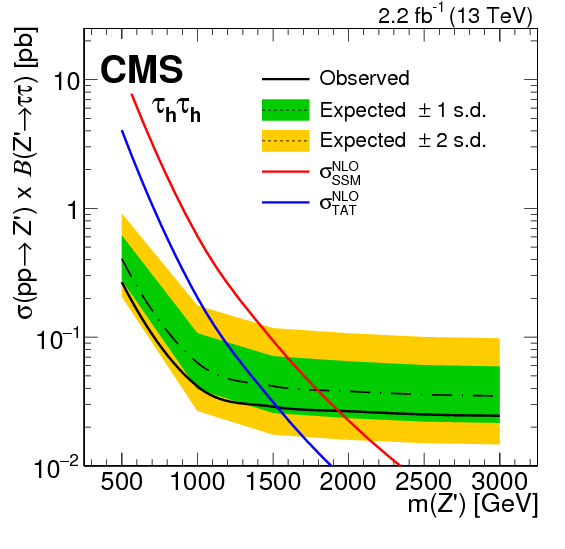
\includegraphics[clip,width=0.45\textwidth]{figuras/Chapter1/CMSZprime2ditauhRun2.png}
 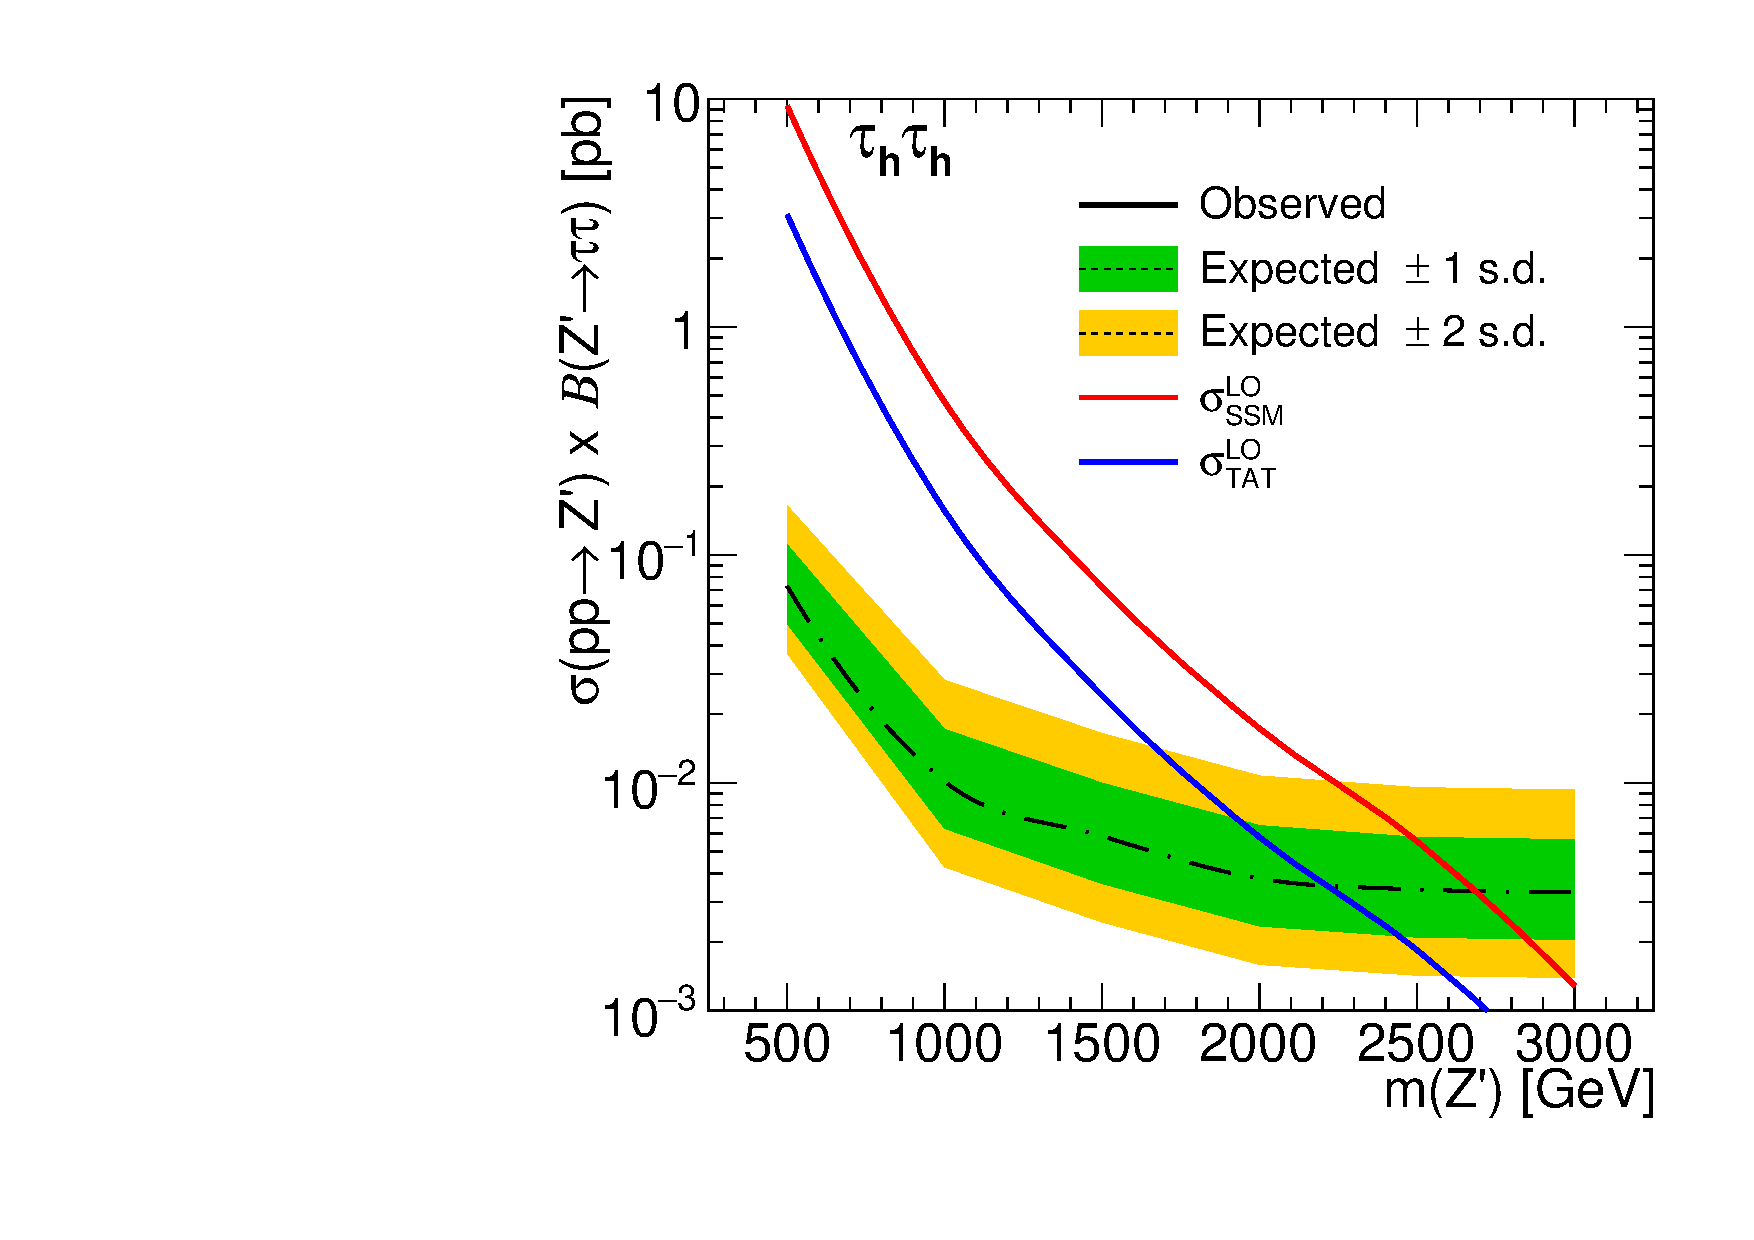
\includegraphics[clip,width=0.45\textwidth]{figuras/Conclusions/tt_Limits.pdf}
 % }
 \end{center}
 \caption{Exclusion limits observed in the search for \Zprimetotauh, using the data collected by CMS during 2015 (left)
 and 2016 (right).}
 \label{fig:ComparisonCMStau}
 \end{figure}

\noindent The main difference between the searches for \Zprime~performed by 
CMS in 2015 and 2016 is the integrated luminosity: 2.2 fb$^{-1}$ for the 2015 run 
and 35.9 fb$^{-1}$ for the 2016 run. In the particular case of the \tauh\tauh~channel, the main differences, besides
luminosity, were exclusion of the so-called pZeta cut (that was used for the 2015 case
and it is defined in Appendix \ref{chap:EventSelection}) and the inclusion 
of the $\cos \Delta\phi(\tau_{lead},\not\!\!E_T)$ cut for the 2016 analysis. The 
$\cos \Delta\phi(\tau_{lead},\not\!\!E_T)$ cut improved the significance  (see Appendix \ref{chap:EventSelection}),
which is reflected in tighter exclusion limits. Figure \ref{fig:ComparisonCMS} shows the comparison between the 
the exclusion limits observed, combining the four di-tau channels, with the 2015 data
(left), and the expected exclusion limits obtained, in the di-hadronic tau channel, with the 2016 data (right). The figure 
shows that the sensitivity in the di-hadronic tau channel, using the 2016 data, is even higher 
that the one obtained with the combination of all four di-tau channels, using the 2015 data. 

\begin{figure}[ht]
 \begin{center}
 \captionsetup[subfloat]{farskip=0pt,captionskip=0.0cm,labelformat=empty}
 % \resizebox{\textwidth}{8.8cm}{
%   \includegraphics[clip,width=0.45\textwidth]{figuras/Chapter1/CMSZprime2ditauRun2.png}
  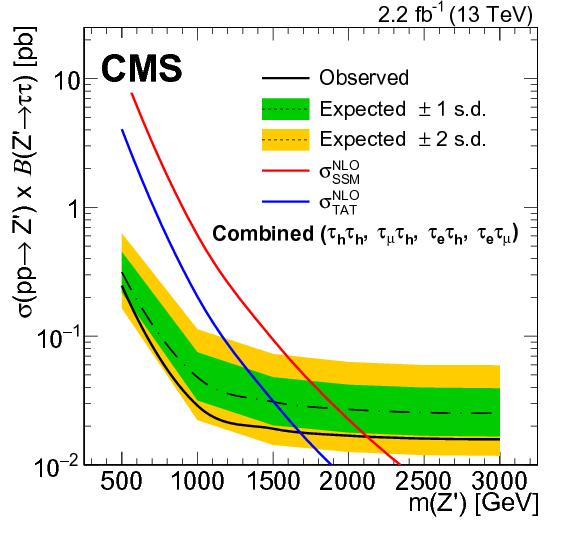
\includegraphics[clip,width=0.45\textwidth]{figuras/Chapter1/CMSZprimeditauRun2.png}
 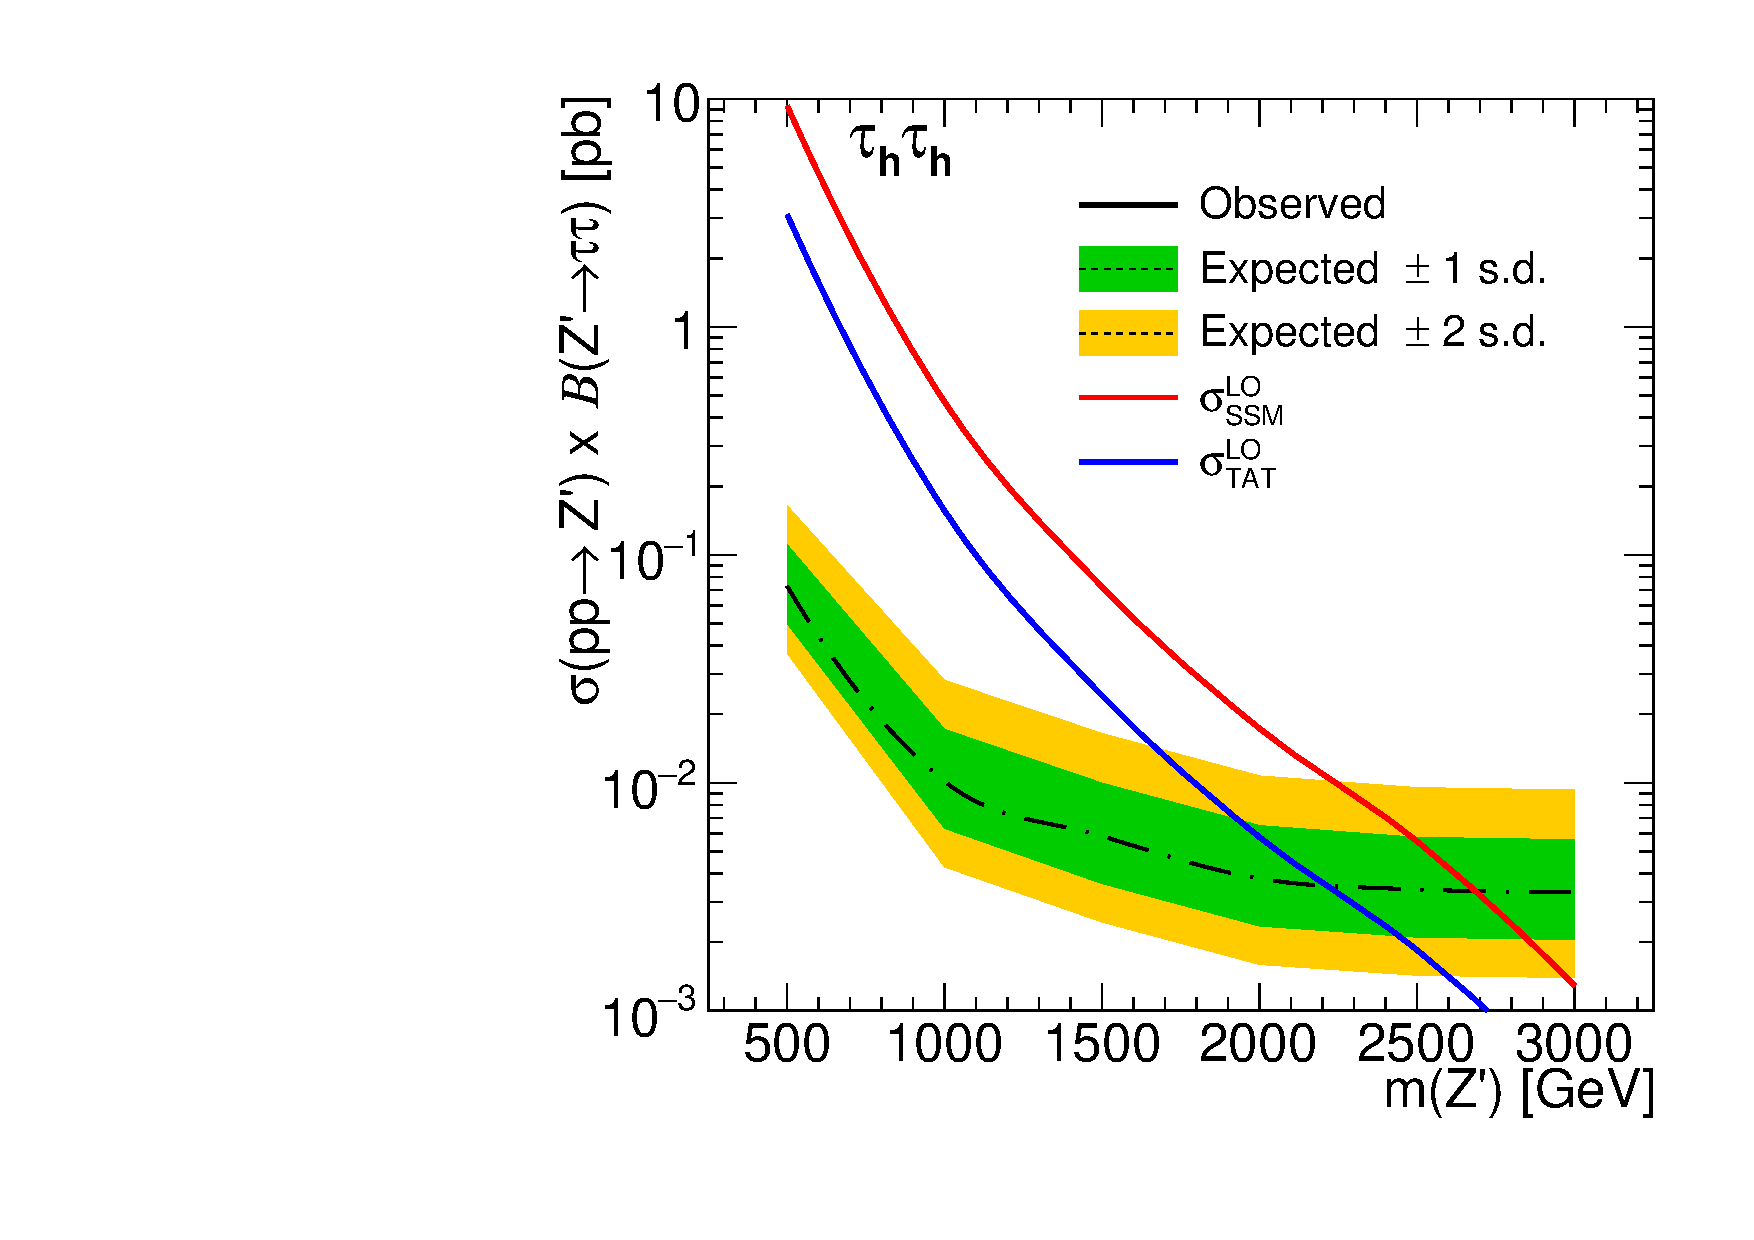
\includegraphics[clip,width=0.45\textwidth]{figuras/Conclusions/tt_Limits.pdf}
 % }
 \end{center}
 \caption{Exclusion limits observed combining the four \Zprimetotautau~channels, using the data collected by CMS during 2015 (left).
 Expected exclusion limits obtained in the search for \Zprimetotauh, using the data collected by CMS during 2016 (right).}
 \label{fig:ComparisonCMS}
 \end{figure}

\subsection{Comparison with Results from ATLAS}
\label{ATLAS}

The search for \Zprime~bosons decaying into taus performed by the ATLAS Collaboration,
using the data collected during 2015 and 2016, with an integrated luminosity 36.1 fb$^{-1}$, 
excluded the \ZprimeSSM~for masses below 2.42 \TeV~at 95 $\%$ CL (see Section \ref{subsec:DirectSearches}). The search 
was performed for the \tauh\tauh, \tauh\taumu~and \tauh\taue~channels. Therefore, the results of this work show
that if no signal is observed in our analysis in CMS, we would obtain significantly higher exclusion 
limits (see Figure \ref{fig:ComparisonATLAS})

\begin{figure}[ht]
 \begin{center}
 \captionsetup[subfloat]{farskip=0pt,captionskip=0.0cm,labelformat=empty}
 % \resizebox{\textwidth}{8.8cm}{
%  \includegraphics[clip,width=0.45\textwidth]{figuras/Chapter1/figure2.pdf}
  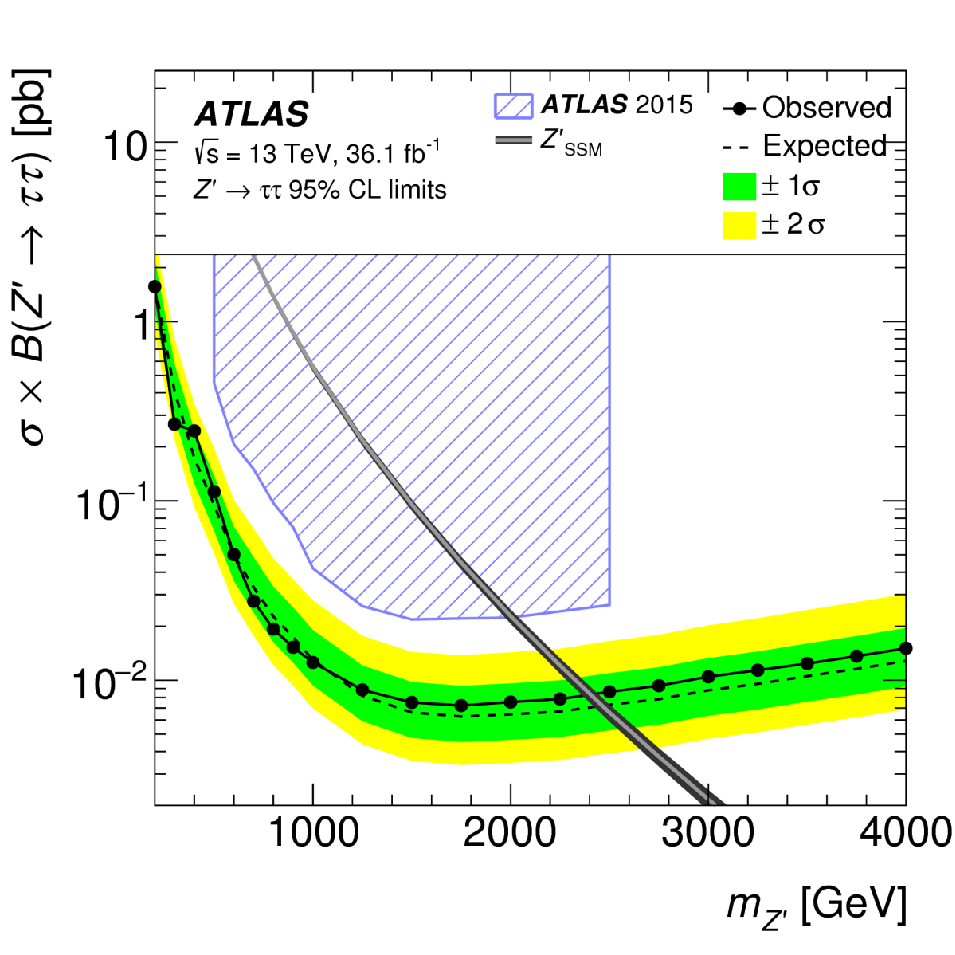
\includegraphics[clip,width=0.45\textwidth]{figuras/Chapter1/ATLASZprime2ditaufigure}
  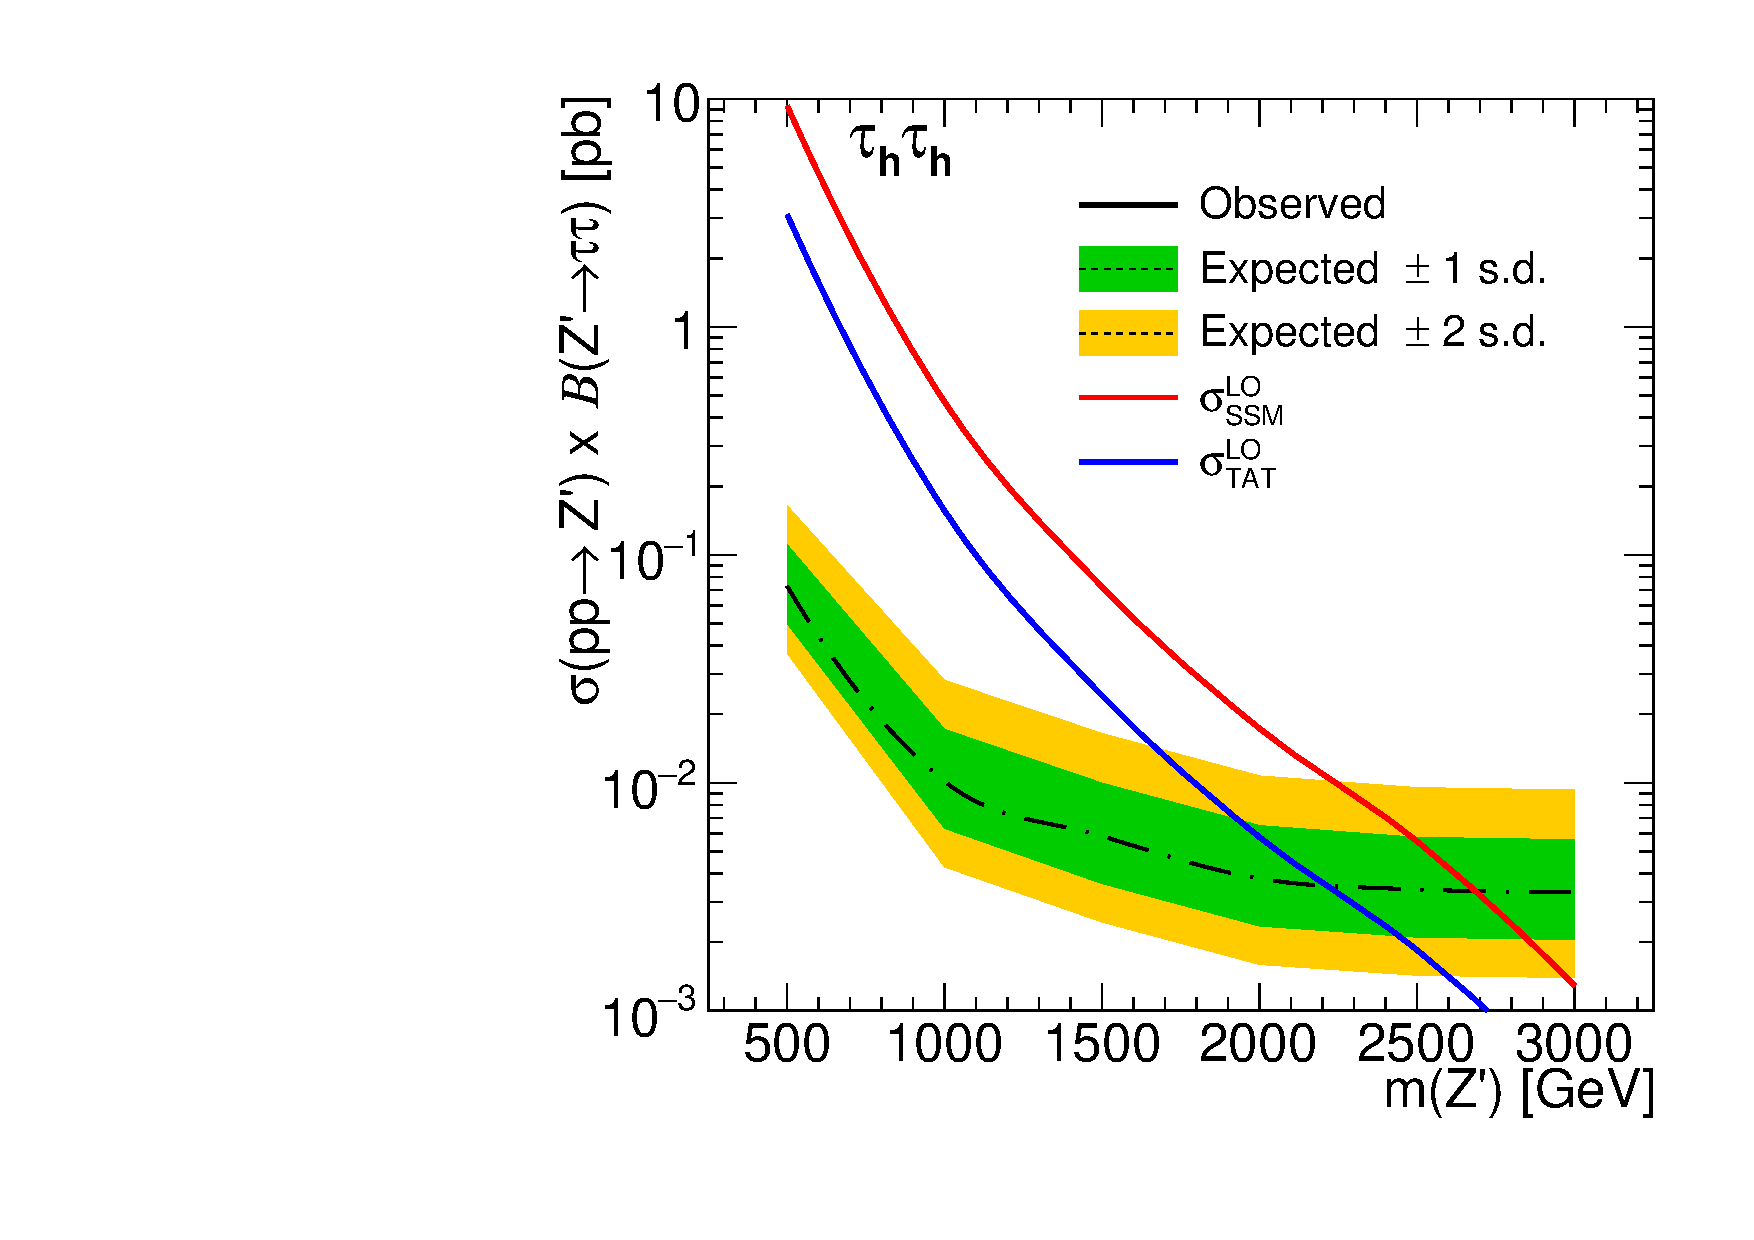
\includegraphics[clip,width=0.45\textwidth]{figuras/Conclusions/tt_Limits.pdf}
 % }
 \end{center}
 \caption{Exclusion limits observed combining the four \Zprimetotautau~channels, using the data collected by ATLAS during 2015 and 2016 (left). 
 Expected exclusion limits obtained in the search for \Zprimetotauh, using the data collected by CMS during 2016 (right).}
 \label{fig:ComparisonATLAS}
 \end{figure}

\section{Conclusions}

\begin{itemize}
 \item In this work a search for \Zprime~bosons decaying into hadronic taus was performed. The search used 
 the data collected by CMS during 2016 of proton-proton collisions at a \centermassenergy~of 13 \TeV~with an 
 integrated luminosity of 35.9 fb$^{-1}$.
 \item Since at this stage (end of May of 2018) no real data has been used yet only expected 
 exclusion limits can be quoted.
 \item The expected exclusion limits obtained in this work are: \mass $~>$ 2.7 \TeV~for \ZprimeSSM~at 95$\%$ CL;
 \mass $~>$ 2.2 \ZprimeTAT~at 95$\%$ CL.
 \item The analysis presented in this work has already been approved by the CMS Collaboration and, therefore, 
 real data can be used to search for a signal or set observed exclusion limits. This analysis is being executed
 and the results should be available for publication very soon (one or two months).
 \item The expected exclusion limits obtained in this work are significantly higher than those 
 obtained during 2015 data and those obtained by ATLAS during 2015 and 2016 data. Therefore, 
 if no signal is observed, as already announce by the ATLAS Collaboration, this analysis will 
 represent an improvement on the previous ones.
 \item The higher sensitivity of this analysis was due mostly to improvements in the selection criteria used.
 \item The Tau identification criteria used in this analysis is slightly different from the one 
 recommended by the CMS TauPOG. However, the results are statistically equivalent.
 \item The excluded exclusion limits quoted in this work corresponds to generic theoretical models (SSM and TAT). However,
 since the kinetic part of the analysis is model independent, it would suggest that for any \Zprime masses below 
 2.2 \TeV~are most likely excluded.
 \end{itemize}
% 
%  agregar un item en el cual se podria la mejora en sensitividad dada la estadistica que se va a alcanzar. estender la exclusion limit hasta 3Tev oor ejemplo y 
%  y en la alta luminosidad hasta 4Tev por ejemplo.


%  
% 1a. se hizo esto se hizo lo otro \\
% 
% b. mejoras con respecto a los otros\\
% 
% 2. limites de exclusion, hasta tales masas, constraints. desfavorecidos unos modelos que otros. BUSCAR \\
% 
% 3. Expectativas. perspectivas, analisis con esta energia y con esta luminosidad, la siguiente version es tal o tal. b-tagging o tau.\\
% 
